\documentclass[12pt, A4]{report}

\usepackage{graphicx}
\graphicspath{{./images/}}

\usepackage{hyperref}
\hypersetup{
    colorlinks=true,
    linkcolor=blue,
    filecolor=magenta,      
    urlcolor=cyan,
}

\urlstyle{same}


\title{\textbf{Decesion Tree}}
\author{Sahasra Ranjan}
\date{April 2020}

\begin{document}

\begin{titlepage}
\maketitle
\end{titlepage}

A decesion tree is a map of the possible outcomes of a series of a related choices. It allows to weigh possible actions against one another based of various factors.\par
It uses a tree-like model of decesion. It typically starts with a single node, which branches into possible outcomes. Each of those outcomes leads to additional nodes, which branch off into other possiblities. 

\begin{figure}[h]
	\centering
	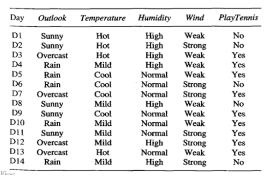
\includegraphics[width=6cm, height=4cm]{dtdata1.png}
	\caption{Dataset for possiblity of a tennis match}
	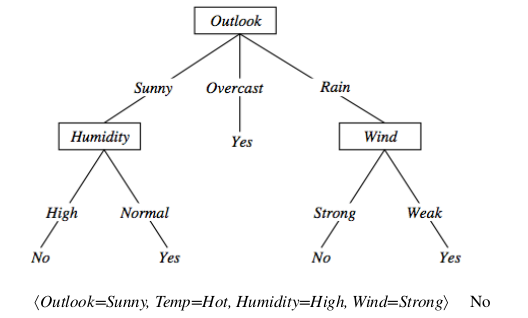
\includegraphics[width=8cm, height=5cm]{dtdata2.png}
	\caption{Decesion Tree for the same}
\end{figure}

\subsection*{Advantages and Disadvantages of Decesion Trees}
	\textbf{Advantages:}
	\begin{itemize}
		\item Performs classification without requiring much computation.
		\item Provides clear indication of important fields for prediction of classification.
	\end{itemize}
	\vspace{15mm}
	\textbf{Disadvantages:}
	\begin{itemize}
		\item Less appropriate for predicting continious attributes.
		\item Computationally expensive to train
	\end{itemize}

\vspace{5mm}
\subsection*{Creating a Decesion Tree}
	For every node, we have to create subtrees with all the possiblities. and then further repeat for other features.\par
	For eg., In the tennis match problem, for the first node  let's check outlook, since having three possiblity (viz. Sunny, Overcast, Rainy), we created three subtrees and then further we keep asking for other features like Humidity \& wind to get the final tree.  

\vspace{5mm}
\subsection*{Greedy Approach for creating decesion tree}
	Greedy approach is implemented by making an optimal local choice at each node. By making these local optimal choices, we reach the approximate optimal solution globaly.

	The algorithm can be summarized as: 
	\begin{enumerate}
		\item At each stage (node), pick out the best feature as the test conditiion.
		\item Now split the node into possibel outcomes (internal nodes)
		\item Repeat the above steps till all the test conditions have been exhausted into leaf nodes.
	\end{enumerate}

\vspace{5mm}
\subsection*{Continuous Features}
	There might be some feature which are not categorical, for these we need to create possibilities on the basis of aprropriate ranges. One such tree is shown below:
	\begin{figure}[h]
		\centering
		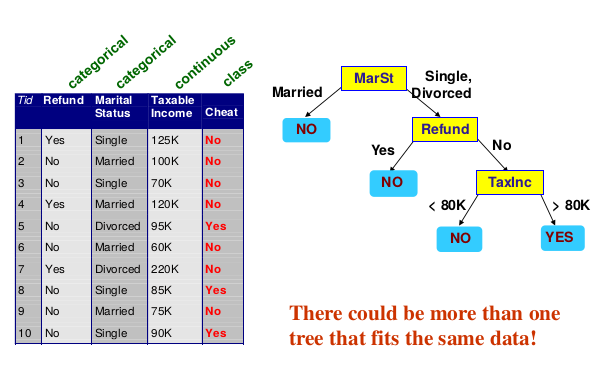
\includegraphics[width=12cm, height=6cm]{continuousDT.png}
		\caption{Decesion tree with continuous feature}
	\end{figure}


\subsection*{Entropy}
	In the most layman terms, Entropy is nothing but the \textbf{The measure of disorder}.
	Why is it important to study entropy for machine learning? \\
	\\ Entropy is a measure of disorder or uncertainity and the goal of machine learning models and Data Scientists in general is to reduce uncertainity.\\
	\\ The Mathematical formula for entropy is - 
	\begin{equation}\label {eq:entropy}
		E(S) = \sum_{i=1}^c - p_i log_2 p_i\
	\end{equation}
	Where $p_i$ is the frequentist probability of an element/class $i$ in out data.\\
	\\ Let's say we have only two classes, a positive and a negative class. Out of 100 data, suppose that 70 belongs to $-$ve class and 30 to $+$ve. Then, P$+$ will be 0.3 and P$-$ will be 0.7.
	\vspace{4mm}
	Entropy $E$ will be given by:
	\begin{equation}
		E = -\frac{3}{10} \times log_2{\frac{3}{10}}-\frac{7}{10} \times log_2{\frac{7}{10}} \approx \textbf{0.88}
	\end{equation}
	\begin{figure}[h]
		\centering
		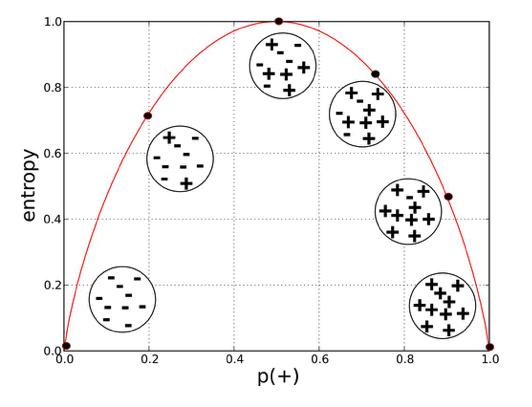
\includegraphics[width=8cm, height=6cm]{entropyDT.png}
		\caption{Entropy distribution frequentist probability}
	\end{figure}

\subsection*{Information Gain}
	Information gain is basically how much Entropy is removed after training a decesion tree.\\
	\textbf{Higher information gain = more entropy removed.}\\
	In technical terms, Information Gain from X on Y is defined as:
	\begin{equation}\label{eq:inforamtion gain}
		IG(Y,X) = E(Y) - E(Y|X)
	\end{equation}
	Basics of inforation gain is well explained here: \href{https://victorzhou.com/blog/information-gain/}{A Simple Explanation of Information Gain and Entropy}

\subsection*{Example: Decesion Tree}
	Consider an example where we are building a decision tree to predict whether a loan given to a person would result in a write-off or not. Our entire population consists of 30 instances. 16 belong to the write-off class and the other 14 belong to the non-write-off class. We have two features, namely “Balance” that can take on two values: “$<$ 50K” or “$>$ 50K” and “Residence” that can take on three values: “OWN”, “RENT” or “OTHER”. I’m going to show you how a decision tree algorithm would decide what attribute to split on first and what feature provides more information, or reduces more uncertainty about our target variable out of the two using the concepts of Entropy and Information Gain.
	\begin{figure}[h]
		\centering
		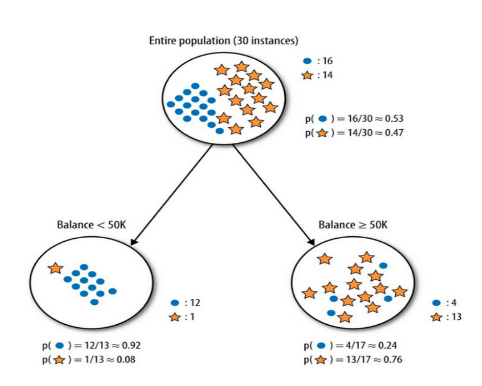
\includegraphics[width=10cm, height=7.5cm]{tree1.png}
		\caption{Feature 1: Balance}
	\end{figure}
	The dots are the data points with class right-off and the stars are the non-write-offs. Splitting the parent node on attribute balance gives us 2 child nodes. The left node gets 13 of the total observations with 12/13 ( 0.92 probability) observations from the write-off class and only 1/13( 0.08 probability) observations from the non-write of class. The right node gets 17 of the total observation with 13/17( 0.76 probability) observations from the non-write-off class and 4/17 ( 0.24 probability) from the write-off class.
	\\ \\Let’s calculate\footnote[1]{See this for calculations and further refrences: \href{https://towardsdatascience.com/entropy-how-decision-trees-make-decisions-2946b9c18c8}{Entropy: How Decesion Trees Make Decesions}} the entropy for the parent node and see how much uncertainty the tree can reduce by splitting on Balance.	
	Splitting on feature ,“Balance” leads to an information gain of 0.37 on our target variable. Let’s do the same thing for feature, “Residence” to see how it compares.\\ 
	\begin{figure}[h]
		\centering
		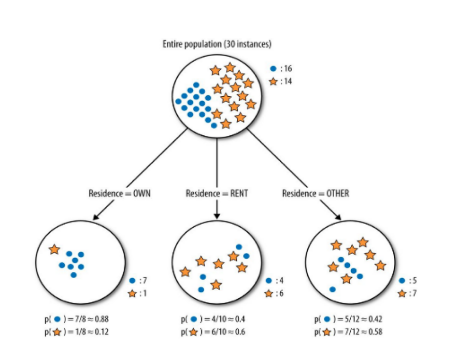
\includegraphics[width=10cm, height=7.5cm]{tree2.png}
		\caption{Feature 2: Residence}
	\end{figure}
	\\
	Splitting the tree on Residence gives us 3 child nodes. The left child node gets 8 of the total observations with 7/8 (0.88 probability) observations from the write-off class and only 1/8 (0.12 probability) observations from the non-write-off class. The middle child nodes gets 10 of the total observations with 4/10 (0.4 probability) observations of the write-off class and 6/10( 0.6 probability) observations from the non-write-off class. The right child node gets 12 of the total observations with 5/12 ( 0.42 probability) observations from the write-off class and 7/12 ( 0.58 ) observations from the non-write-off class. We already know the entropy for the parent node. We simply need to calculate the entropy after the split to compute the information gain from “Residence”

	The information gain from feature, Balance is almost 3 times more than the information gain from Residence! If you go back and take a look at the graphs you can see that the child nodes from splitting on Balance do seem purer than those of Residence. However the left most node for residence is also very pure but this is where the weighted averages come in play. Even though that node is very pure, it has the least amount of the total observations and a result contributes a small portion of it’s purity when we calculate the total entropy from splitting on Residence. This is important because we’re looking for overall informative power of a feature and we don’t want our results to be skewed by a rare value in a feature.
	\\ \\
	By itself the feature, Balance provides more information about our target variable than Residence. It reduces more disorder in our target variable. A decision tree algorithm would use this result to make the first split on our data using Balance. From here on, the decision tree algorithm would use this process at every split to decide what feature it is going to split on next. In a real world scenario , with more than two features the first split is made on the most informative feature and then at every split the information gain for each additional feature needs to be recomputed because it would not be the same as the information gain from each feature by itself. The entropy and information gain would have to be calculated after one or more splits have already been made which would change the results. A decision tree would repeat this process as it grows deeper and deeper till either it reaches a pre-defined depth or no additional split can result in a higher information gain beyond a certain threshold which can also usually be specified as a hyper-parameter!
\\ \\
	There you have it! You now know what entropy and information gain are and how they are computed. You understand how a decision tree either by itself or in a tree based ensemble decides on the best order of features to split on and decides when to stop when it trains itself on given data. If you every have to explain the intricacies of how decision trees work to someone, hopefully you won’t do too bad.\\

\end{document}